\documentclass[12pt]{article}
%%%%%%%%%%%%%%%%
% Packages
%%%%%%%%%%%%%%%%

\usepackage[top=2cm,bottom=2cm,left=2cm,right= 2cm]{geometry}
\usepackage[parfill]{parskip}
\usepackage{graphicx, fontspec, xcolor,multicol, enumitem, setspace, amsmath, changepage}
\DeclareGraphicsRule{.tif}{png}{.png}{`convert #1 `dirname #1`/`basename #1 .tif`.png}

%%%%%%%%%%%%%%%%
% User defined colors
%%%%%%%%%%%%%%%%

% Pantone 2015 Fall colors
% http://iwork3.us/2015/02/18/pantone-2015-fall-fashion-report/
% update each semester or year

\xdefinecolor{custom_blue}{rgb}{0, 0.32, 0.48} % FROM SPRING 2016 COLOR PREVIEW
\xdefinecolor{custom_darkBlue}{rgb}{0.20, 0.20, 0.39} % Reflecting Pond  
\xdefinecolor{custom_orange}{rgb}{0.96, 0.57, 0.42} % Cadmium Orange
\xdefinecolor{custom_green}{rgb}{0, 0.47, 0.52} % Biscay Bay
\xdefinecolor{custom_red}{rgb}{0.58, 0.32, 0.32} % Marsala

\xdefinecolor{custom_lightGray}{rgb}{0.78, 0.80, 0.80} % Glacier Gray
\xdefinecolor{custom_darkGray}{rgb}{0.35, 0.39, 0.43} % Stormy Weather

%%%%%%%%%%%%%%%%
% Color text commands
%%%%%%%%%%%%%%%%

%orange
\newcommand{\orange}[1]{\textit{\textcolor{custom_orange}{#1}}}

% yellow
\newcommand{\yellow}[1]{\textit{\textcolor{yellow}{#1}}}

% blue
\newcommand{\blue}[1]{\textit{\textcolor{blue}{#1}}}

% green
\newcommand{\green}[1]{\textit{\textcolor{custom_green}{#1}}}

% red
\newcommand{\red}[1]{\textit{\textcolor{custom_red}{#1}}}

%%%%%%%%%%%%%%%%
% Coloring titles, links, etc.
%%%%%%%%%%%%%%%%

\usepackage{titlesec}
\titleformat{\section}
{\color{custom_blue}\normalfont\Large\bfseries}
{\color{custom_blue}\thesection}{1em}{}
\titleformat{\subsection}
{\color{custom_blue}\normalfont}
{\color{custom_blue}\thesubsection}{1em}{}

\newcommand{\ttl}[1]{ \textsc{{\LARGE \textbf{{\color{custom_blue} #1} } }}}

\newcommand{\tl}[1]{ \textsc{{\large \textbf{{\color{custom_blue} #1} } }}}

\usepackage[colorlinks=false,pdfborder={0 0 0},urlcolor= custom_orange,colorlinks=true,linkcolor= custom_orange, citecolor= custom_orange,backref=true]{hyperref}

%%%%%%%%%%%%%%%%
% Instructions box
%%%%%%%%%%%%%%%%

\newcommand{\inst}[1]{
\colorbox{custom_blue!20!white!50}{\parbox{\textwidth}{
	\vskip10pt
	\leftskip10pt \rightskip10pt
	#1
	\vskip10pt
}}
\vskip10pt
}

%%%%%%%%%%%
% App Ex number    %
%%%%%%%%%%%

% DON'T FORGET TO UPDATE

\newcommand{\appno}[1]
{3.2}

%%%%%%%%%%%%%%
% Turn on/off solutions       %
%%%%%%%%%%%%%%

% Off
\newcommand{\soln}[2]{$\:$\\ \vspace{#1}}{}

%%% On
%\newcommand{\soln}[2]{\textit{\textcolor{custom_red}{#2}}}{}

%%%%%%%%%%%%%%%%
% Document
%%%%%%%%%%%%%%%%

\begin{document}
\fontspec[Ligatures=TeX]{Helvetica Neue Light}

Dr. \c{C}etinkaya-Rundel \hfill Sta 101: Data Analysis and Statistical Inference \\
Duke University - Department of Statistical Science \hfill \\

\ttl{Application exercise \appno{}: \\
Grade inflation}

\inst{$\:$ \\
Team name: \rule{10cm}{0.5pt} \\
$\:$ \\
Lab section: $\qquad$ 8:30 $\qquad$ 10:05 $\qquad$ 11:45 $\qquad$ 1:25 $\qquad$ 3:05$\qquad$ 4:40 \\
$\:$ \\
Write your responses in the spaces provided below. WRITE LEGIBLY and SHOW ALL WORK! 
Only one submission per team is required. One team will be randomly selected and their 
responses will be discussed and graded. Concise and coherent are best!}

%%%%%%%%%%%%%%%%%%%%%%%%%%%%%%%%%%%%

In 2001 the average GPA of students at Duke University was 3.37. Last semester 63 Sta 101 
students responded to the question on GPA on the class survey. The mean was 3.58, and the 
standard deviation 0.53. A histogram of the data is shown below.

\begin{center}
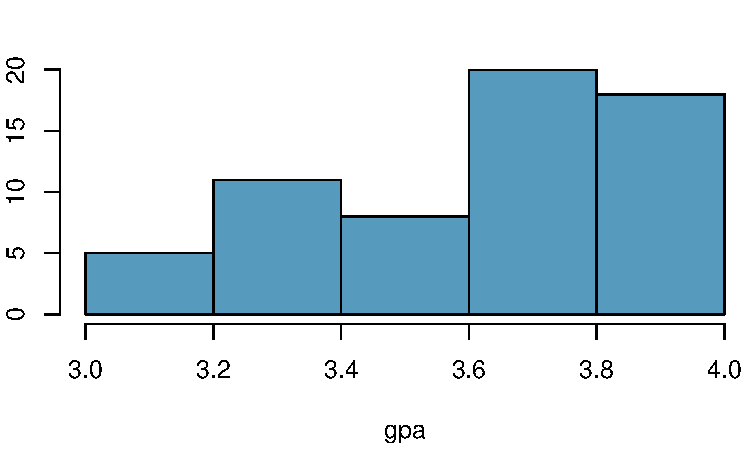
\includegraphics[width=0.5\textwidth]{survey/hist_gpa}
\end{center}

Assuming that this sample is random and representative of all Duke students (bit of a leap 
of faith? you can discuss that when checking the conditions), do these data provide 
convincing evidence that the average GPA of Duke students has \textbf{\underline{changed}} 
over the last decade and a half?

Make sure to check conditions, note any assumptions you make, and show all your work.

\soln{4cm}{
Conditions:
\begin{itemize}
\item The sample is less than 10\% of the population of all Duke students, however it is not random.
It may not be reasonable to assume that the GPAs of sampled Duke students are independent
of each other.
\item The distribution is not extremely skewed, and the sample size is sufficiently large, to yield a nearly
normal sampling distribution of the mean.
\end{itemize}
\[ Z = \frac{3.58 - 3.37}{0.53 / \sqrt{63}} = 3.15 \rightarrow p-value = 0.0016 \]
}

%%%%%%%%%%%%%%%%%%%%%%%%%%%%%%%%%%%%

\end{document}